\documentclass[12pt]{report}

\usepackage[a4paper]{geometry}
\usepackage[utf8]{inputenc}
\usepackage[portuguese]{babel}
\usepackage{graphicx}

\newcommand\tab[1][0.5cm]{\hspace*{#1}}

\title{Projeto de Sistemas Operativos (MiEI) \\ 2017/2018}
\author{Alexandre Mendonça Pinho (a82441) \and Joel Filipe Esteves Gama (a82202) \and Tiago Martins Pinheiro (a82491)}
\date{\today}

\begin{document}
\maketitle

\tableofcontents

\chapter{Introdução}
\label{sec:introducao}

\tab Neste projeto é-nos proposto construir um sistema para processamento de notebooks, que misturam fragmentos de código, resultados da execução, e documentação. Estes notebooks, tratam-se de ficheiros de texto, que depois de processados, são modificados de modo a incluir resultados da execução de código ou comandos nele embebidos.

\chapter{Descrição do projeto}
\label{sec:descricao}

\tab Para resolver o problema que nos foi apresentado começamos por fazer o parsing do ficheiro. O parsing excluí o output dos comandos e constroi o grafo de execução. Num grafo de execução os nodos correspondem a comandos e as arestas são os redicionamentos dos comandos. Se um nodo A do grafo tem uma aresta vinda de um nodo B significa que o output de B será redirecionado como o input de A, se o nodo for isolado ou não tiver arestas vindas de outros nodos significa que o comando recebe o input do standard input. Já o que é para escrever no ficheiro final é mantido em memória central com recurso a uma lista ligada de strings.

Depois do parsing passamos para a execução dos comandos. Cada comando cria um pipe que é usado para distribuir o output do comando. A distribuição é feita através do programa distribuidor que lê do pipe e escreve nos fifos onde o output é necessário.

No final da execução de cada comando os outputs são colocados na lista ligada de strings, (cada comando tem um índice que indica qual a posição onde deve ser adicionado na lista ligada) que está em memória central, para serem escritos em ficheiro.
\chapter{Exemplo}

\label{sec:exemplo}

Ficheiro de input exemplo:

\texttt{
\newline
    Listagem da diretoria atual\newline
    \$ ls\newline
\newline
    O número de ficheiros na listagem\newline
    \$ | wc -l\newline
\newline
    O nome do primeiro elemento\newline
    \$ 2 | head -1\newline
\newline
    Aceitar input do utilizador\newline
    \$ cat
}

\begin{figure}
    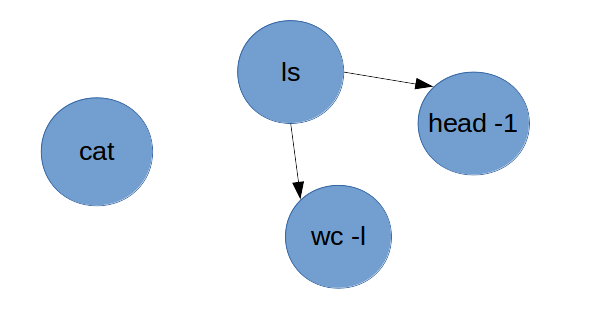
\includegraphics[width=\linewidth]{grafo_execucao_exemplo.png}
    \caption{Grafo de execução}
    \label{fig:grafo_execucao}
\end{figure}

\begin{figure}
    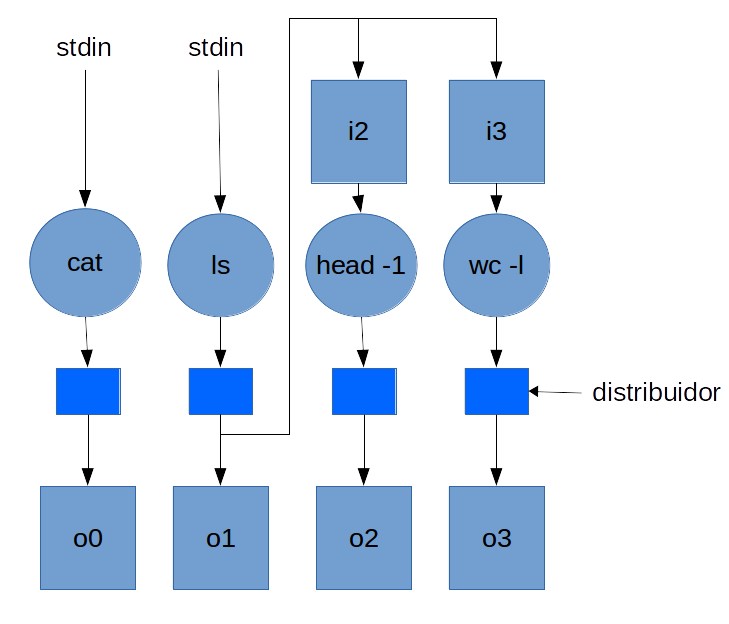
\includegraphics[width=\linewidth]{esquema_execucao_exemplo.png}
    \caption{Esquema de execução}
    \label{fig:esquema_execucao}
\end{figure}

\noindent Ficheiro de output resultante, ao introduzir pelo no teclado o string "Hello, world!\textbackslash n":

\texttt{
\newline Listagem da diretoria atual
\newline \$ ls
\newline >>>
\newline distribuidor \newline distribuidor.c \newline i1 \newline i2
\newline include \newline lib \newline main.c \newline Makefile
\newline notebook \newline o0 \newline o1 \newline o2 \newline o3
\newline obj \newline README.md \newline relatorio \newline test
\newline <<<
\newline O número de ficheiros na listagem
\newline \$ | wc -l
\newline >>>
\newline 17
\newline <<<
\newline O nome do primeiro elemento
\newline \$ 2 | head -1
\newline >>>
\newline distribuidor
\newline <<<
\newline Aceitar input do utilizador
\newline \$ cat
\newline >>>
\newline Hello, world!
\newline <<<
\newline
}

\chapter{Conclusão}
\label{sec:conclusao}

\tab Foi-nos prosposto, como projeto de avaliação, conceber um sistema que fosse capaz de processar \textit{notebooks}, através da sua leitura e  interpretação. A implementação foi feita na linguagem de programação \textit{C}, utilizando os conceitos aprendidos durante as aulas práticas ao longo do semestre. 

Para os métodos de comunicação entre processos, escolhemos pipes anónimos para comunicar entre os processos e os distribuidores, e \textit{fifos} para comunicar entre os diferentes processos através dos distribuidores. Assim, a comunicação entre processos é tratada de forma simples pelos distribuidores.

\end{document}
